% Faithful, searchable reconstruction of the six supplied examination pages.
% Student identification fields are intentionally blank.
\examsetup{September 29, 2016}{Fall 2016}
\begingroup
\vspace*{1.15in}
\begin{center}
{\sffamily\bfseries\fontsize{16}{19}\selectfont Texas A\&M University\\
Department of Electrical and Computer Engineering\par}
\vspace{.38in}
{\sffamily\bfseries\fontsize{15}{18}\selectfont
ECEN 474/704 -- (Analog) VLSI Circuit Design\par}
\vspace{.38in}
{\sffamily\bfseries\fontsize{15}{18}\selectfont Fall 2016\par}
\vspace{.34in}
{\sffamily\bfseries\fontsize{15}{18}\selectfont Exam \#1\par}
\vspace{.34in}
{\sffamily\bfseries\fontsize{15}{18}\selectfont Instructor: Sam Palermo\par}
\end{center}
\vspace{.37in}
\begin{itemize}[leftmargin=.3in,itemsep=0pt,topsep=0pt]
\item Please write your name in the space provided below
\item Please verify that there are \textbf{6 pages} in your exam
\item You may use \underline{one double-sided page} of notes and equations for the exam
\item Good Luck!
\end{itemize}
\vspace{.58in}
\begin{tabular}{|c|c|c|}
\hline Problem&Score&Max Score\\\hline
1&&40\\\hline 2&&40\\\hline 3&&20\\\hline
\textbf{Total}&&\textbf{100}\\\hline
\end{tabular}
\vfill
Name:\ \hrulefill\par
\vspace{.11in}
UIN:\ \hrulefill
\vspace{.18in}
\newpage

\begingroup
\fontsize{10.95}{12.5}\selectfont
\setlength{\parskip}{4pt}
\textbf{Problem 1 (40 points)}\par
\textbf{For the layout below, assume that all the commonly labeled diffusion areas are connected with the appropriate metal layers. Assume that
$V_A=2\,\mathrm V$, $V_B=1.2\,\mathrm V$, $V_C=0\,\mathrm V$,
$V_D=1.2\,\mathrm V$, $V_E=2\,\mathrm V$, $V_{T0}=0.7\,\mathrm V$,
$\gamma=0$, and that all Spice parameters are given (i.e. $C_j$, $C_{jsw}$,
$C_{jc}$, $C_{ox}$, $C_{ov}$). The dimensions are given in $\mu\mathrm m$,
with the poly gates having an $L_D=0.1\,\mu\mathrm m$.}
\begin{enumerate}[label=\alph*),leftmargin=.24in,itemsep=0pt,topsep=1pt]
\item Draw the equivalent circuit. Combine all parallel transistors and give the total width and length of the equivalent transistors.
\item What region(s) are the transistors operating in?
\item \textbf{For node B only}, give an expression and calculate the total gate cap.
\item \textbf{For node D only}, give an expression and calculate the total junction cap, including the relevant channel--bulk cap. Note for the perimeter terms, include the sides underneath the gate.
\end{enumerate}
\vspace{2pt}
\begin{minipage}[t]{.52\linewidth}
\centering
\begin{tikzpicture}[x=.105cm,y=.105cm,font=\scriptsize]
\draw (-5,-8) rectangle (70,34);
\fill[gray!70] (3,30) rectangle (5,32);
\node[anchor=west] at (6,31) {Poly};
\fill[black] (26,30) rectangle (28,32);
\node[anchor=west] at (29,31) {Contact (poly or diff.)};
\fill[pattern=crosshatch dots] (3,25) rectangle (5,27);
\node[anchor=west] at (6,26) {N+};
\fill[gray!20] (26,25) rectangle (28,27);
\node[anchor=west] at (29,26) {M1};
\node[anchor=west] at (0,20) {P-sub};
% All diffusion strips have height 10 and exposed widths of 6 micrometers.
\fill[gray!15] (0,-1) rectangle (66,11);
\fill[pattern=crosshatch dots] (0,0) rectangle (66,10);
\draw (0,0) rectangle (66,10);
% M1 connects the A diffusion contact to the upper poly rail and the
% B diffusion contact to the lower poly rail. Black squares below are vias.
\fill[gray!20] (1.5,6) rectangle (4.5,17);
\fill[gray!20] (9.5,-5.5) rectangle (12.5,4);
\fill[gray!20] (9.5,-5.5) rectangle (18.5,-2.5);
\foreach \x/\w in {6/2,14/6,26/6,38/2,46/2,54/6}{
  \fill[gray!70] (\x,-1) rectangle ++(\w,12);
  \draw (\x,-1) rectangle ++(\w,12);
}
\fill[gray!70] (6,10) rectangle (8,16);
\fill[gray!70] (1.5,14) rectangle (48,16);
\fill[gray!70] (38,10) rectangle (40,16);
\fill[gray!70] (46,10) rectangle (48,16);
\fill[gray!70] (14,-5) rectangle (20,0);
\fill[gray!70] (26,-5) rectangle (32,0);
\fill[gray!70] (54,-5) rectangle (60,0);
\fill[gray!70] (14,-5) rectangle (60,-3);
\foreach \x/\lab in {3/A,11/B,23/C,35/D,43/E,51/D,63/C}{
  \fill (\x-1,2) rectangle (\x+1,4);
  \fill (\x-1,6) rectangle (\x+1,8);
  \node[fill=white,inner sep=.1pt] at (\x,5) {\lab};
}
\fill (2,14) rectangle (4,16);
\fill (16,-5) rectangle (18,-3);
\draw[<->] (-2,0)--node[left]{10}(-2,10);
\foreach \x/\lab in {3/6,7/2,11/6,17/6,23/6,29/6,35/6,39/2,43/6,47/2,51/6,57/6,63/6}
  \node[font=\tiny] at (\x,-1.8) {\lab};
\end{tikzpicture}

\raggedright
\textbf{(a) Parallel combinations.}
The six consecutive devices along the strip are
\[
\begin{array}{c|cccccc}
\text{terminals}&A\!:\!B&B\!:\!C&C\!:\!D&D\!:\!E&E\!:\!D&D\!:\!C\\
W/L&10/2&10/6&10/6&10/2&10/2&10/6
\end{array}
\]
Combining the parallel $C$--$D$ and $D$--$E$ devices gives the circuit at right. All $W/L$ values are drawn dimensions in $\mu\mathrm m/\mu\mathrm m$.

\textbf{(b) Operating regions.}
For $M_1$,
\[
V_{GS}=V_{DS}=1.2\,\mathrm V>V_T,
\quad V_{DS}>V_{GS}-V_T.
\]
Hence $M_1$ is in saturation. $M_3$ has the same voltages and is also in saturation.
For $M_2$,
\[
V_{GS}=V_{DS}=0.8\,\mathrm V>V_T,
\quad V_{DS}>V_{GS}-V_T.
\]
Thus $M_2$ and, similarly, $M_4$ are in saturation.
\end{minipage}\hfill
\begin{minipage}[t]{.455\linewidth}
\centering
\begin{circuitikz}[scale=.85,transform shape,font=\small]
\node[nmos] (m1) at (1,0) {};
\node[nmos] (m2) at (1,2.1) {};
\node[nmos] (m3) at (4.1,0) {};
\node[nmos] (m4) at (4.1,2.1) {};
\draw (m1.D)--(m2.S) coordinate[midway](b);
\draw (m3.D)--(m4.S) coordinate[midway](d);
\draw (m1.S)--++(0,-.4) coordinate(c)--(m3.S |- c)--(m3.S);
\draw (c) node[ground]{} node[left]{$C=0\,\mathrm V$};
\draw (m2.D)--++(0,.4) coordinate(a) node[above]{$A=2\,\mathrm V$};
\draw (m4.D)--++(0,.4) node[above]{$E=2\,\mathrm V$};
\draw (m2.G)--++(-.45,0)|-(a);
\draw (m1.G)--++(-.45,0)|-(b);
\draw (m4.G)--++(-.4,0) coordinate(ga);
\draw (a)--++(1.2,0)-|(ga);
\draw (m3.G)--++(-.4,0) coordinate(gb);
\draw (b)--++(1.2,0)-|(gb);
\node[above right,fill=white,inner sep=1pt]at(b){$B=1.2\,\mathrm V$};
\node[right]at(d){$D=1.2\,\mathrm V$};
\node[left]at(m1.S){$M_1:\ 10/6$};
\node[left]at(m2.S){$M_2:\ 10/2$};
\node[right]at(m3.S){$M_3:\ 20/6$};
\node[right]at(m4.S){$M_4:\ 20/2$};
\end{circuitikz}

\raggedright
\textbf{(c) Gate capacitance at B.}
For $M_1$, its gate--drain overlap is shorted out because both terminals are at B. With $L_{\rm eff}=6-2L_D=5.8\,\mu\mathrm m$,
\begin{align*}
C_{gB,M_1}
&=\frac23(10)(5.8)\,\mu\mathrm m^2C_{ox}
  +10\,\mu\mathrm m C_{ov}\\
&\simeq38.7\,\mu\mathrm m^2C_{ox}
  +10\,\mu\mathrm m C_{ov}.
\end{align*}
For $M_3$, both overlap capacitors contribute:
\begin{align*}
C_{gB,M_3}
&=\frac23(20)(5.8)\,\mu\mathrm m^2C_{ox}
  +2(20)\,\mu\mathrm m C_{ov}\\
&\simeq77.3\,\mu\mathrm m^2C_{ox}
  +40\,\mu\mathrm m C_{ov}.
\end{align*}
\[
\boxed{C_{gB}=116\,\mu\mathrm m^2C_{ox}
       +50\,\mu\mathrm m C_{ov}.}
\]
\end{minipage}

\textbf{(d) Junction capacitance at D.}
The two D diffusion regions each have area $6\times10\,\mu\mathrm m^2$ and perimeter $2(6+10)\,\mu\mathrm m$, including the gate-adjacent edges. Add the channel--bulk term of $M_4$, with $L_{\rm eff}=2-2L_D=1.8\,\mu\mathrm m$:
\begin{align*}
C_{jD}&=A_D C_j+P_D C_{jsw}+C_{cb,M_4}\\
&=(6)(10)(2)\,\mu\mathrm m^2C_j
 +(6+10)(2)(2)\,\mu\mathrm m C_{jsw}
 +\frac23(20)(1.8)\,\mu\mathrm m^2C_{jc}\\
&=\boxed{120\,\mu\mathrm m^2C_j+64\,\mu\mathrm m C_{jsw}
        +24\,\mu\mathrm m^2C_{jc}.}
\end{align*}
\endgroup
\newpage

\textbf{Problem 2 (40 points)}\par
\textbf{For the circuit shown below, the transistor is operating in a fully velocity saturated region where its DC drain current is given exactly by the given equation.}
\begin{enumerate}[label=\alph*.,leftmargin=.23in,topsep=0pt,itemsep=0pt]
\item Draw the low-frequency small-signal model of the circuit (neglecting transistor capacitors) and give an expression for the small-signal voltage gain of the circuit, $A_v=v_o/v_i$, as a function of the relevant transistor conductances and the load resistor. Note, you can assume that the input AC-coupling capacitor acts as an ideal short.
\end{enumerate}
\begin{minipage}[t]{.35\linewidth}
\vspace{0pt}
\centering
\begin{circuitikz}[scale=.85,transform shape]
\node[nmos,bulk] (m) at (0,0) {};
\draw (m.D) to[R,l={$R_D=1\,\mathrm{k}\Omega$}] ++(0,2) node[vcc]{};
\draw (m.D)--++(1,0) node[right]{$V_D+v_o$};
\draw (m.G)--++(-.8,0) node[left]{$1\,\mathrm V$};
\draw (m.S)--++(0,-.35) coordinate(s) to[I,l_=$I_B$] ++(0,-1.5) node[ground]{};
\draw (s) to[C] ++(2,0) to[sV,l=$v_i$] ++(0,-1.5) node[ground]{};
\node[below right]at(s){$V_S$};
\draw (m.bulk)--++(.6,0) node[right]{$0.4\,\mathrm V$};
\node at(-.8,-.65){$\dfrac{W}{1\,\mu\mathrm m}$};
\end{circuitikz}
\end{minipage}\hfill
\begin{minipage}[t]{.62\linewidth}
\vspace{0pt}
\[
I_{DS}=v_{sat}C_{ox}W(V_{GS}-V_{Tn})
\]
\[
V_{Tn}=V_{T0}+\gamma\left(
\sqrt{|2\Phi_F|+V_{SB}}-\sqrt{|2\Phi_F|}\right).
\]
\solutionlabel
There is no $V_{DS}$ dependence in the stated model, so $g_{ds}=0$ and $r_o=\infty$.

\begin{circuitikz}[scale=.75,transform shape,font=\small]
\draw (0,0) to[sV,l=$v_i$] (0,1.5)--(4.2,1.5);
\draw (0,0) node[ground]{};
\draw (0,3.5) to[cI] (0,1.5);
\draw (0,3.5)--(4.2,3.5) node[right]{$v_o$};
\draw (2.2,3.5) to[cI] (2.2,1.5);
\node[above]at(0,3.8){$g_m(-v_i)$};
\node[above]at(2.2,3.8){$g_{mb}(-v_i)$};
\draw (4.2,3.5) to[R,l=$R_D$] (4.2,0) node[ground]{};
\end{circuitikz}
\end{minipage}
\begin{align*}
g_m&=\frac{\partial I_D}{\partial V_{GS}}=v_{sat}C_{ox}W,\\
g_{mb}&=\frac{\partial I_D}{\partial V_{BS}}
=v_{sat}C_{ox}W(-1)(-1)
\frac{\gamma}{2\sqrt{|2\Phi_F|+V_{SB}}}
=\eta g_m,\\
\eta&=\frac{\gamma}{2\sqrt{|2\Phi_F|+V_{SB}}}.
\end{align*}
\[
v_o=-(g_m+g_{mb})(-v_i)R_D,
\qquad\boxed{A_v=\frac{v_o}{v_i}=(g_m+g_{mb})R_D.}
\]
\vspace{.15in}
\begin{enumerate}[label=\alph*.,start=2,leftmargin=.23in,topsep=0pt]
\item Assume the following DC operating points for the drain and source voltages,
$V_{S,Q}=0.2\,\mathrm V$ and $V_{D,Q}=1\,\mathrm V$, and that
$v_{sat}C_{ox}=250\,\mu\mathrm A/(\mathrm V\cdot\mu\mathrm m)$,
$V_{T0}=0.7\,\mathrm V$, $\gamma=0.45\,\mathrm V^{1/2}$,
$2\Phi_F=0.9\,\mathrm V$, and $L_D=0.1\,\mu\mathrm m$.
Calculate the necessary transistor width $W$ for $|A_v|=5\,\mathrm{V/V}$.
\end{enumerate}
\solutionlabel
Here $V_{SB}=0.2-0.4=-0.2\,\mathrm V$. Consequently,
\[
\eta=\frac{0.45}{2\sqrt{0.9-0.2}}\simeq0.269.
\]
\[
A_v=(1+\eta)g_mR_D=(1+\eta)v_{sat}C_{ox}WR_D,
\]
\[
\boxed{W=\frac{A_v}{(1+\eta)v_{sat}C_{ox}R_D}
=\frac5{(1.269)(250\,\mu\mathrm A/(\mathrm V\cdot\mu\mathrm m))
             (1\,\mathrm{k}\Omega)}\simeq15.8\,\mu\mathrm m.}
\]
\newpage

\textbf{Problem 3 (20 points)}\par
\textbf{a.\quad Poly resistor design}\par
Design and sketch a layout of a $500\,\Omega$ poly resistor. Assume that the poly
$R_{\square}=60\,\Omega/\square$, each $(1\,\mu\mathrm m\times1\,\mu\mathrm m)$
contact has resistance of $10\,\Omega$, and fabrication tolerances limit the minimum
unit resistor width $W\ge3\,\mu\mathrm m$. Use at least 2 fingers in the resistor
design. In the sketch clearly label the critical dimensions.

\solutionlabel
\[
R_{\rm total}=\left(\frac{2R_c}{n}+R_{\square}\frac LW\right)F,
\qquad
\begin{array}{l}
n=\text{number of parallel contacts per end},\\
F=\text{number of fingers (unit resistors)}.
\end{array}
\]
\[
L=\left(\frac{R_{\rm total}}F-\frac{2R_c}n\right)\frac W{R_{\square}}.
\]
Set $W=3\,\mu\mathrm m$, $n=3$, and $F=2$. Then
\[
L=\left(\frac{500}2-\frac{2(10)}3\right)
  \left(\frac{3\,\mu\mathrm m}{60}\right)
  \simeq\boxed{12.2\,\mu\mathrm m}.
\]
\begin{center}
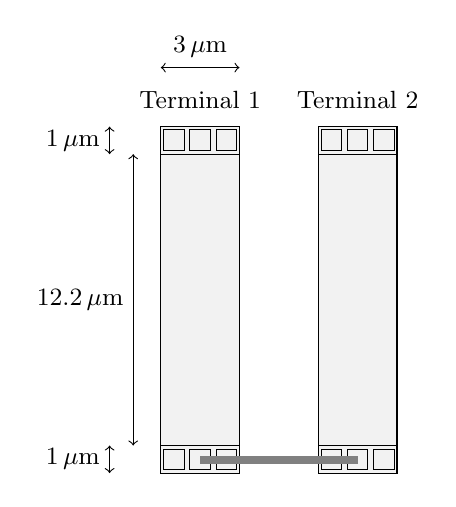
\begin{tikzpicture}[x=1cm,y=1cm,font=\small]
\foreach \x in {0,2}{
  \fill[gray!10] (\x,0) rectangle ++(1,4.4);
  \draw (\x,0) rectangle ++(1,4.4);
  \draw (\x,.35)--++(1,0);
  \draw (\x,4.05)--++(1,0);
  \foreach \dx in {.1667,.5,.8333}{
    \draw (\x+\dx-.13,.04) rectangle ++(.26,.26);
    \draw (\x+\dx-.13,4.10) rectangle ++(.26,.26);
  }
}
\draw[line width=3pt,gray] (.5,.17)--(2.5,.17);
\draw[<->] (0,5.15)--node[above]{$3\,\mu\mathrm m$}(1,5.15);
\draw[<->] (-.35,.35)--node[left]{$12.2\,\mu\mathrm m$}(-.35,4.05);
\draw[<->] (-.65,0)--node[left]{$1\,\mu\mathrm m$}(-.65,.35);
\draw[<->] (-.65,4.05)--node[left]{$1\,\mu\mathrm m$}(-.65,4.4);
\node[above]at(.5,4.5){Terminal 1};
\node[above]at(2.5,4.5){Terminal 2};
\end{tikzpicture}
\end{center}
{\small The source rounds the calculated body length $12.1667\,\mu\mathrm m$ to $12.2\,\mu\mathrm m$; the capacitance below uses that rounded drawn dimension.}

\vspace{.2in}
\textbf{b.\quad Poly resistor parasitic capacitance}\par
The poly resistor has a parallel-plate parasitic capacitance to substrate of
$0.1\,\mathrm{fF}/\mu\mathrm m^2$. What is the total parasitic capacitance of the
resistor? Include the contact area in the capacitance calculation and assume
that the capacitance is only due to the parallel-plate effect, i.e. neglect
any fringing capacitance.

\solutionlabel
\[
\text{Resistor area}=(12.2\,\mu\mathrm m+2\,\mu\mathrm m)
 (3\,\mu\mathrm m)(2)=86.4\,\mu\mathrm m^2.
\]
\[
\boxed{C_{\rm parasitic}=(86.4\,\mu\mathrm m^2)
       (0.1\,\mathrm{fF}/\mu\mathrm m^2)=8.64\,\mathrm{fF}.}
\]
\newpage

\textbf{c.\quad N-well resistor design}\par
Design and sketch a layout of a $500\,\Omega$ n-well resistor. Assume that the n-well
$R_{\square}=2\,\mathrm{k}\Omega/\square$, each
$(1\,\mu\mathrm m\times1\,\mu\mathrm m)$ contact has resistance of $10\,\Omega$,
and fabrication tolerances limit the minimum unit resistor length $L\ge6\,\mu\mathrm m$.
Use at least 2 fingers in the resistor design. In the sketch clearly label the critical dimensions.

\solutionlabel
\[
R_{\rm total}=\left(\frac{2R_c}{n}+R_{\square}\frac LW\right)F,
\qquad
L=\left(\frac{R_{\rm total}}F-\frac{2R_c}n\right)\frac W{R_{\square}}.
\]
Set $F=2$, $W=50\,\mu\mathrm m$, and $n=50$. Thus
\[
L=\left(\frac{500}2-\frac{2(10)}{50}\right)
\left(\frac{50\,\mu\mathrm m}{2000}\right)
=\boxed{6.24\,\mu\mathrm m}.
\]
\begin{center}
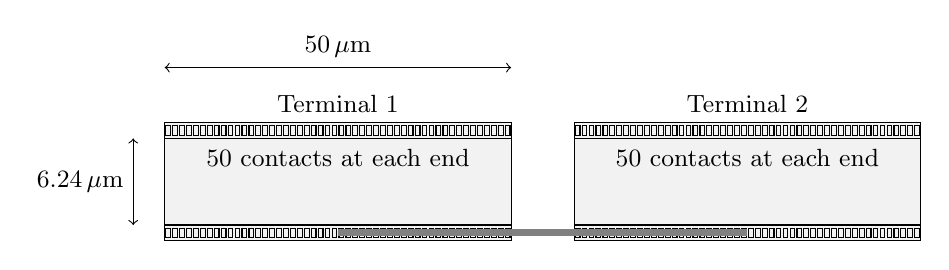
\begin{tikzpicture}[x=1cm,y=1cm,font=\small]
\foreach \x in {0,5.2}{
  \fill[gray!10] (\x,0) rectangle ++(4.4,1.5);
  \draw (\x,0) rectangle ++(4.4,1.5);
  \draw (\x,.2)--++(4.4,0);
  \draw (\x,1.3)--++(4.4,0);
  \foreach \i in {0,...,49}{
    \pgfmathsetmacro{\xx}{\x+.044+.088*\i}
    \draw (\xx-.03,.04) rectangle ++(.06,.12);
    \draw (\xx-.03,1.34) rectangle ++(.06,.12);
  }
}
\draw[line width=2.5pt,gray] (2.2,.1)--(7.4,.1);
\draw[<->] (0,2.2)--node[above]{$50\,\mu\mathrm m$}(4.4,2.2);
\draw[<->] (-.4,.2)--node[left]{$6.24\,\mu\mathrm m$}(-.4,1.3);
\node at(2.2,1.05){50 contacts at each end};
\node at(7.4,1.05){50 contacts at each end};
\node[above]at(2.2,1.51){Terminal 1};
\node[above]at(7.4,1.51){Terminal 2};
\end{tikzpicture}
\end{center}

\vspace{.45in}
\textbf{d.\quad N-well resistor parasitic capacitance}\par
The n-well resistor has a parallel-plate parasitic capacitance to substrate of
$1\,\mathrm{fF}/\mu\mathrm m^2$. What is the total parasitic capacitance of the
resistor? Include the contact area in the capacitance calculation and assume
that the capacitance is only due to the parallel-plate effect, i.e. neglect
any fringing capacitance.

\solutionlabel
\[
\text{Resistor area}=(6.24\,\mu\mathrm m+2\,\mu\mathrm m)
(50\,\mu\mathrm m)(2)=824\,\mu\mathrm m^2.
\]
\[
\boxed{C_{\rm parasitic}=(824\,\mu\mathrm m^2)
       (1\,\mathrm{fF}/\mu\mathrm m^2)=824\,\mathrm{fF}.}
\]
\par\vspace{.25in}
\textbf{e.\quad If we have to use the $500\,\Omega$ resistor for a high-frequency
application, which design should we choose, the poly or n-well design? Why?}

\solutionlabel
Choose the \textbf{poly resistor}: it has less parasitic capacitance.
\newpage

\begin{center}
{\sffamily\bfseries\fontsize{17}{20}\selectfont Scratch Paper}
\end{center}
\vfill
\null
\clearpage
\endgroup
